\documentclass[11pt]{beamer}
\usepackage[utf8]{inputenc}
\usepackage[T1]{fontenc}
\usepackage{lmodern}
\usepackage[english, serbian]{babel}
\usepackage{graphicx}
\usepackage{color}
\usepackage{beamerthemeshadow}
\usepackage{hyperref}
\usepackage[flushleft]{threeparttable}
\definecolor{beamer@darkred}{rgb}{0.76,0.23,0.13}
\setbeamercolor{structure}{fg=beamer@darkred}
\usetheme{Frankfurt}
%\logo{\includegraphics[height=1.5 cm]{logo.png}}

\begin{document}
\author{\small{Nikolina Šobić, Marina Stanojlović, Anja Nenadović, Maša Kočinac}}
	\title{Prednosti i mane onlajn učenja}
	\subtitle{-Seminarski rad iz predmeta Tehničko i naučno pisanje"-}
	\institute{Matematički fakultet\\Univerzitet u Beogradu}
	\date{
		\footnotesize{Beograd, 2022.}	
}

\begin{frame}[plain]
		\maketitle
\end{frame}
	
	
	\addtocounter{framenumber}{-1}
	
\begin{frame}[fragile]
		\frametitle{Literatura}
		 Na osnovu sledeće literature:\\
		\begin{itemize}
	
		\item
		    Online nastava u visokom obrazovanju – prednosti, nedostaci i izazovi – Jelena Matijašević, Marko Carić, Sanja Škorić; Univerzitet Privredna akademija, Pravni fakultet za privredu i pravosudje, Novi Sad, Srbija
		
		\item
		    Prednosti i nedostaci online nastave iz ugla profesora i saradnika – Tatjana Pivac, Milica Pavkov Hrvojević, Lana Zorić; Univerzitet u Novom Sadu, Prirodno-matematički fakultet, Novi Sad, Srbija
		
		\item
    	    Online education in Malaysia: THE GOOD, THE BAD, THE UGLY AND THE WAY FORWARD, Muzaffar Syah Mallow and Syed Saddiq Syed Abdul Rahman
		
		
		
		\item
		     Opažanja studenata o iskustvu onlajn nastave tokom pandemije Covid-19 - Vasiljevic Danica - Markovic Zagorka
		
		\item
		       Rezultati-istrazivanje-o-stavovima-mladih-o-onlajn obrazovanju-u-Srbiji
		
		
		\end{itemize}
\end{frame}


\begin{frame}
		\frametitle{Pregled}
		\tableofcontents[hidesubsections] 

\end{frame}



\begin{frame}
		\frametitle{Uvod}
		\section{Uvod}
		
		\small{	
    \textbf{Učenje na daljinu} je, u stvari, mnogo starije od učenja putem interneta. Ovakav način učenja postojao je mnogo pre nego što su ljudi znali za računar i internet.
  
    U različitim periodima svog razvoja odvijalo se korišćenjem različitih tehnologija kao što su poštanski sistem, radio, televizija i naposletku internet.
   
    \underline{E-učenje} je oblik nastave gde predavači putem savremenih informacionih tehnologija podučavaju učenike/studente. To je interaktivan proces koji je upotpunjen medijima kao pomoćnim sredstvom.}
\end{frame}
	
	
\begin{frame}
		\frametitle{Prednosti}
		\section{Prednosti}
  \begin{itemize}
		
		\subsection{Prednost 1}\item[1.]{Prva prednost koju je vredno spomenuti je da onlajn učenje omogućava više \underline{slobode}.}
        \subsection{Prednost 2}\item[2.]{Materijali sa predavanja su dostupni 24 časa dnevno.
        Svako može raditi odgovarajućom brzinom.}
         \subsection{Prednost 3}\item[3.]{Postoji bezbroj aplikacija koje profesori mogu iskoristiti za interakciju tokom učenja.}
         \subsection{Prednost 4}\item[4.]{Prilikom realizacije onlajn nastave, danas najpopularnijeg vida učenja na daljinu, razvijaju se \underline{digitalne veštine}, kako kod profesora, tako i kod studenata.}
         \end{itemize}
         
\end{frame}

\begin{frame}
		\frametitle{Mane}
		\section{Mane}
		
		\begin{itemize}
	\subsection{Mana 1}\item[1.]{Među najčešćim problemima ili lošim stranama u realizaciji online obrazovanja je nedostatak objekata za sprovođenje online obrazovanja i
    loše online veštine među samim učiteljima i učenicima. }

	\subsection{Mana 2}
		
	\item[2.]{ \underline{Povratne informacije} učenika prilično su ograničene.}
 \subsection {Mana 3}\item[3.] {Proces učenja na daljinu zahteva visok nivo samomotivacije i discipline. \underline{Odsutnost samomotivacije i nedisciplina} mogu postati glavna prepreka
na putu uspeha učenika. }
		\end{itemize}
	
\end{frame}





\begin{frame}
		\frametitle{Stavovi mladih o učenju na daljinu}
		\section{Stavovi mladih o učenju na daljinu}
		\subsection{Istraživanje i rezultati}
		Upitnik se sastojao od opšteg dela kojim se prikupljaju osnovni podaci o ispitanicima (pol, nivo i godina studija, zaposlenost i boravište) i skalera od 19 tvrdnji koje se odnose na kvalitet onlajn nastave.\\ Upitnik sadrži tri podskale: Nastavno prisustvo (7 tvrdnji), Socijalno prisustvo (6 tvrdnji) i Kognitivnoprisustvo (6 tvrdnji). Ispitanici su označavali stepen slaganja ili neslaganja sa ponuđenim tvrdnjama na petostepenoj skali.
\end{frame}

\parskip=\baselineskip
\begin{table}
\centering
\parskip=\baselineskip
  \begin{tabular}{ | l | c | r |}
    \hline
    \textbf{pol} & \textbf{vrednost} & \textbf{procenat} \\ \hline
    muški & 7 & 7,7 \\ \hline 
    ženski & 84 & 92,3 \\ \hline
    ukupno & 91 & 100 \\
    \hline
  \end{tabular}
  \caption{Struktura ispitanika prema polu}
\end{table}

\begin{table}
\parskip=\baselineskip
\centering
  \begin{tabular}{ | l | c |}
    \hline
    \textbf{Mišljenje} & \textbf{Frekvencija} \\ \hline
    da, potpuno & 13  \\ \hline 
    delimično, kombinovanje je najbolje & 27  \\ \hline
    ne, tradicionalno je bolje & 20  \\ \hline
    nisam siguran & 31 \\ \hline
    ukupno &  91 \\
    \hline
  \end{tabular}
  \caption{Da li online nastava može zameniti tradicionalnu nastavu?}
\end{table}


\begin{frame}
	\begin{itemize}
		\only<1>{\item Slika 1}
		\only<2>{\item Slika 2}
		\only<3>{\item Slika 3}
	\end{itemize}
		\centering
		\begin{figure}[h!]
		\only<1>{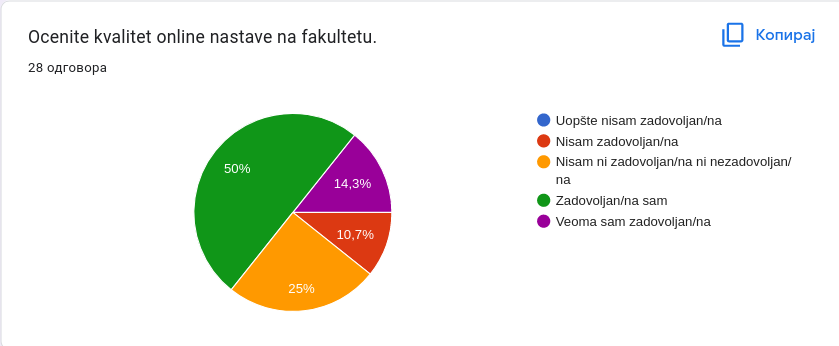
\includegraphics[width=0.6\textwidth]{1.png}
		\caption{Ocenjivanje kvaliteta nastave}
        \label{fig:slika1}}
		\only<2>{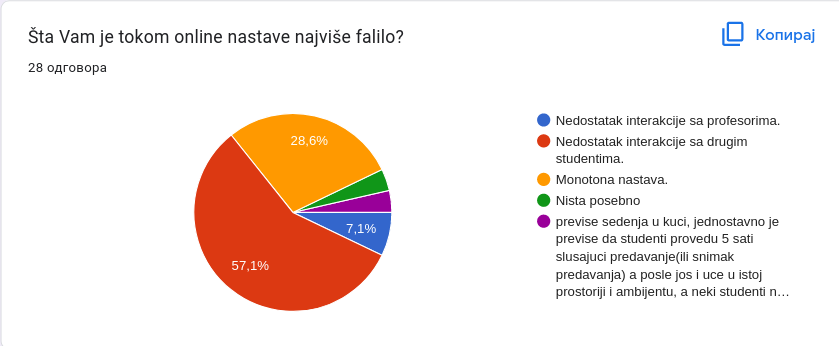
\includegraphics[width=0.7\textwidth]{2.png}
		\caption{Nedostaci onlajn nastave}}
		\label{fig:slika2}
		\only<3>{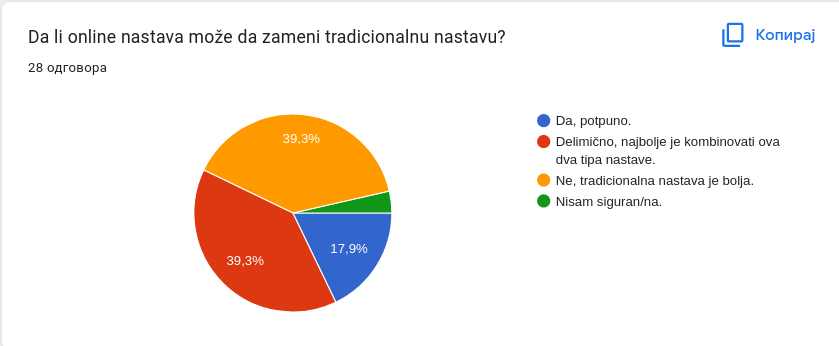
\includegraphics[width=0.7\textwidth]{3.png}
		\caption{Odnos onlajn i tradicionalne nastave}}
		\end{figure}
\end{frame}


\begin{frame}
    \frametitle{Zaključak}
		\section{Zaključak}
		     Ljudi su oduvek imali potrebu da stiču nova znanja, pa su bili prinudjeni da se prilagode raznim situacijama kako bi u toj nameri i uspeli.\\ Prirodno je postaviti pitanje koji je vid učenja najbolji, ali jasno je da \underline{ne postoji univerzalan odgovor}. \\Odgovor na ovo pitanje je individualan i zavisi od ambicija i afiniteta učenika, kao i od mnogo drugih faktora.
		\small{	
  
  }
\end{frame}



\end{document}